\documentclass[aspectratio=169,usenames,dvipsnames]{beamer}

\mode<presentation>{
  \usetheme{default}
  \usecolortheme{default}
  \usefonttheme{default}
}

% ------------------------------------------------
% Colors
% ------------------------------------------------
\usepackage{xcolor}
\definecolor{purple}{HTML}{695693}
\definecolor{navy}{HTML}{567293}
\definecolor{ruby}{HTML}{9a2515}
\definecolor{alice}{HTML}{107895}
\definecolor{daisy}{HTML}{EBC944}
\definecolor{coral}{HTML}{F26D21}
\definecolor{kelly}{HTML}{829356}
\definecolor{cranberry}{HTML}{E64173}
\definecolor{jet}{HTML}{131516}
\definecolor{asher}{HTML}{555F61}
\definecolor{slate}{HTML}{314F4F}
\definecolor{accent}{HTML}{107895}
\definecolor{accent2}{HTML}{9a2515}

\definecolor{blue1}{RGB}{27,  98, 168}
\definecolor{blue2}{RGB}{67, 135, 195}
\definecolor{blue3}{RGB}{114,169, 211}
\definecolor{blue4}{RGB}{169,206, 227}
\definecolor{redUT}{RGB}{215, 48,  39}

% ------------------------------------------------
% Fonts & math
% ------------------------------------------------
\usepackage[T1]{fontenc}
\usepackage{amsmath, amssymb}
\usepackage{setspace}
\usepackage{bbm}

% ------------------------------------------------
% Tables / figures
% ------------------------------------------------
\usepackage{geometry}
\usepackage{float}
\usepackage{booktabs}
\usepackage{multirow}
\usepackage{graphicx}
\usepackage{subfigure}
\usepackage{array}
\usepackage{tabularx}
\usepackage{threeparttable}
\usepackage{makecell}
\newcolumntype{C}{>{\centering\arraybackslash}X}

% ------------------------------------------------
% TikZ
% ------------------------------------------------
\usepackage{tikz}
\usetikzlibrary{calc}
\usetikzlibrary{fit,shapes.misc}
\usetikzlibrary{tikzmark}
\usepackage{colortbl}

% ------------------------------------------------
% Misc
% ------------------------------------------------
\usepackage{comment}
\usepackage{caption}
\usepackage{color}
\usepackage{pdfpages}
% ------------------------------------------------
% Bibliography
% ------------------------------------------------
\usepackage[round, authoryear]{natbib}
\bibliographystyle{chicago}

\newcommand{\smallcite}[1]{{\footnotesize\textcolor{Blue}{\citep{#1}}}}

% ------------------------------------------------
% Hyperref
% ------------------------------------------------
\usepackage{hyperref}
\hypersetup{
    colorlinks=true,
    citecolor=Blue,
    linkcolor=Blue,
    urlcolor=Blue
}

% ------------------------------------------------
% Beamer colors
% ------------------------------------------------
\setbeamertemplate{navigation symbols}{}
\setbeamercolor{frametitle}{fg=Blue}
\setbeamercolor{item projected}{fg=Blue}
\setbeamercolor{title}{fg=Blue}
\setbeamercolor{section in head/foot}{fg=Blue}
\setbeamercolor{subsection in head/foot}{fg=Blue}

% ------------------------------------------------
% Footline
% ------------------------------------------------
\setbeamertemplate{footline}{
  \leavevmode
  \hbox{
  \begin{beamercolorbox}[wd=.333333\paperwidth,ht=2.25ex,dp=1ex,center]{title in foot}
    \usebeamerfont{title in foot}\insertsection
  \end{beamercolorbox}
  \begin{beamercolorbox}[wd=.333333\paperwidth,ht=2.25ex,dp=1ex,center]{date in foot}
    \usebeamerfont{date in foot}\hspace*{2em}
  \end{beamercolorbox}
  \begin{beamercolorbox}[wd=.333333\paperwidth,ht=2.25ex,dp=1ex,right]{number in foot}
    \usebeamerfont{numb in foot}\insertframenumber{}/\inserttotalframenumber{}\hspace*{2em}
  \end{beamercolorbox}}
  \vskip1pt
}

% ------------------------------------------------
% Backup slides
% ------------------------------------------------
\newcommand{\backupbegin}{
   \newcounter{finalframe}
   \setcounter{finalframe}{\value{framenumber}}
}

\newcommand{\backupend}{
   \setcounter{framenumber}{\value{finalframe}}
}

% ------------------------------------------------
% Graphics
% ------------------------------------------------
\graphicspath{{figures/}}

% ------------------------------------------------
% TITLE
% ------------------------------------------------
% ------------------------------------------------
% TITLE
% ------------------------------------------------
\title[W]{\LARGE{Do CCT Programs (Really) Reduce Mortality?\\Ten-Year Evidence from Mexico}}

\author[]{%
  \texorpdfstring{%
    \begin{tabular}{c c c}
      Emma Aguila & William H.\ Dow & Felipe Menares$^{*}$ \\
      \textcolor{gray}{USC} & \textcolor{gray}{UC Berkeley} & \textcolor{gray}{Inter-American Development Bank} \\[4pt]
      Susan W.\ Parker & Jorge Peniche & Soomin Ryu \\
      \textcolor{gray}{University of Maryland} & \textcolor{gray}{USC} & \textcolor{gray}{University of Missouri} \\
    \end{tabular}
  }
  {Emma Aguila, William H. Dow, Felipe Menares, Susan W. Parker, Jorge Peniche, Soomin Ryu}
}

\date{June 2026}

% ------------------------------------------------
% DOCUMENT
% ------------------------------------------------
\begin{document}

\setlength{\abovedisplayskip}{3pt}
\setlength{\belowdisplayskip}{3pt}

\includepdf[pages={1},noautoscale=false,fitpaper=false]{ppt_iadb/Half-baked_Lunch_Backdrop.pdf}

{
\setbeamertemplate{footline}{}
\begin{frame}
  \titlepage
  \vfill
  {\tiny $^{*}$The opinions expressed in this paper are those of the authors and do not necessarily reflect the views of the Inter-American Development Bank, its Board of Directors, or the countries they represent, nor of INEGI.}
\end{frame}
}
\note{Hello everyone. Today I'm presenting joint work on whether Mexico's Progresa conditional cash transfer program reduced elderly mortality. Our paper asks whether a program primarily designed to invest in children's education and health produced meaningful mortality benefits for the elderly over a longer time horizon.}

%%%%%%%%%%%%%%%%%%%%%%%%%%%%%%%%%%%%%%%%
%%% MOTIVATION %%%
%%%%%%%%%%%%%%%%%%%%%%%%%%%%%%%%%%%%%%%%
\section{Background}

\begin{frame}{Motivation: Older adults are the fastest-growing population group}\label{motivation}
\vspace{2pt}
\small
\begin{itemize}
  \item[$\circ$] In LAC, 10\% is 65+, and is expected to double by 2050 (20\%  in poverty) \smallcite{UN2024WPP} 
  \item[$\circ$] Income support programs and health: evidence is mixed
    \begin{itemize}
      \item Some studies find important health benefits \smallcite{Case2004PerspectivesAging, Aguila2015PNAS}, others find no effects \smallcite{LloydSherlockAgrawal2014JDS}, and some identify unintended adverse consequences \smallcite{FernaldGertlerHou2008JN}
    \end{itemize}
  \vspace{4pt}
  \item[$\circ$] Most existing evidence focuses on \textbf{short-run} rather than long-run \textbf{mortality} effects
  \vspace{4pt}
  \item[$\circ$] CCTs have been widely studied for children, but \textbf{elderly} has been overlooked
    \begin{itemize}
      \item improved health-service utilization for elderly women \smallcite{BehrmanParker2013Demography}
      \item higher hypertension diagnosis, but no improvement in biomarkers \smallcite{aguila2024conditional}
      \item
      \textit{short-run} reductions in elderly mortality over first years \smallcite{BarhamRowberry2013JDE}
    \end{itemize}
  \vspace{4pt}
  \item[$\circ$] \textbf{Direct} pension programs for older adults show larger effects
    \begin{itemize}
      \item Mexico's \textit{70 y Más}: $-5.5\%$ elderly women mortality \smallcite{Menares2026JHR}
    \end{itemize}
\end{itemize}
\end{frame}

\note{The broader literature on income transfers and health yields mixed results. Some find benefits, others find none. Most evidence is short-run. For the elderly specifically, we know Progresa increased clinic visits but didn't improve blood pressure biomarkers. Barham and Rowberry provided the key short-run mortality finding. And we know that pension programs that transfer directly to the elderly show stronger effects.}

\begin{frame}{This Paper}\label{thispaper}
\vspace{4pt}
\small
\begin{itemize}
  \item[$\circ$] \textbf{Research question:} Did Mexico's \textit{Progresa} CCT reduce elderly mortality ($65+$) over its first ten years?
  \vspace{6pt}
  \item[$\circ$] \textbf{Identification:} Difference-in-differences exploiting variation in program enrollment intensity across highly marginalized municipalities (1991--2006)
  \vspace{6pt}
  \item[$\circ$] \textbf{Main finding:} \textcolor{redUT}{No evidence of medium- or long-run mortality effects}
    \begin{itemize}
      \item Result is robust to functional form, weighting, and health insurance coverage
    \end{itemize}
  \vspace{6pt}
  \item[$\circ$] \textbf{Revisiting prior evidence:} Short-run estimates of \cite{BarhamRowberry2013JDE} are sensitive to weighting and lag structure
    \begin{itemize}
      \item Minor changes attenuate estimates by $\geq 50\%$
    \end{itemize}
  \vspace{6pt}
  \item[$\circ$] \textbf{Mechanisms:} No significant effects on elderly labor supply, household composition, income, or nutrition
\end{itemize}
\end{frame}

\note{Our paper re-examines this question using fifteen years of vital statistics. The main finding is a null — Progresa did not significantly reduce elderly mortality. We also show that the earlier short-run positive result is fragile: it depends heavily on population weighting and the choice of lag length. And when we look at the channels through which Progresa could have worked, we find no evidence those channels were activated.}

%%%%%%%%%%%%%%%%%%%%%%%%%%%%%%%%%%%%%%%%
%%% PROGRAM BACKGROUND %%%
%%%%%%%%%%%%%%%%%%%%%%%%%%%%%%%%%%%%%%%%
\section{Program}

\begin{frame}{Mexico's \textit{Progresa}: Programme Overview}\label{progresa}
\small
\begin{itemize}
  \item[$\circ$] Launched 1997 in small rural communities and targeted poor households with children under 18 or pregnant women (marginality index and a household-level proxy means test)
  \vspace{4pt}
  \item[$\circ$] \textbf{Scale:} 6 million families covered ($\frac{1}{4}$ of all Mexican families); $\frac{2}{3}$ in rurality
  \vspace{4pt}
  
  \item[$\circ$] \textbf{Transfer:} $\approx$ MXN\$800/month ($>25\%$ income increase); paid to female household head
  \vspace{4pt}
  \item[$\circ$] \textbf{Conditionalities:}
    \begin{itemize}
      \item \textit{Education:} children attend school ($\geq 85\%$ attendance)
      \item \textit{Health:} all family members visit clinic regularly
      \item For adults $17+$ (incl.\ elderly): \textbf{one annual visit only}
    \end{itemize}
  \vspace{4pt}
  \item[$\circ$] \textbf{In 2006:} pension for adults $70+$ added --- we end analysis early to focus on original CCT
  \vspace{4pt}
  \item[$\circ$] \textbf{Elderly in eligible households:}
    \begin{itemize}
      \item $\approx 75\%$ of elderly lived in households with children under 15 \smallcite{BehrmanParker2013Demography}
      \item Most are grandparents --- not direct transfer recipients
      \item Any benefit must come through household income sharing or indirect pathways
    \end{itemize}
\end{itemize}
\end{frame}

\note{Progresa started in 1997 in small rural communities and rapidly scaled. Transfers went to the female head of household. For adults over 17, including elderly, the health conditionality was just one annual clinic visit. This is a very minimal requirement. The elderly in these households are typically grandparents who don't control program funds but might benefit through household resource sharing.}

\begin{frame}{Potential Channels to Elderly Mortality}\label{channels}
\small
\begin{columns}[T]
  \begin{column}{0.48\textwidth}
    \textbf{Theoretical channels}
    \vspace{4pt}
    \begin{enumerate}
      \item \textbf{Health conditionality} \\
        One annual clinic visit $\to$ early detection of diabetes, hypertension, infectious disease
      \vspace{8pt}
      \item \textbf{Income and nutrition} \\
        $+25\%$ household income $\to$ improved nutrition and healthcare access for elderly members
      \vspace{8pt}
      \item \textbf{Living arrangements} \\
        Reduced adult-child migration $\to$ more co-residence and informal caregiving for elderly
    \end{enumerate}
  \end{column}
  \begin{column}{0.48\textwidth}
    \textbf{Why each channel may not work}
    \vspace{4pt}
    \begin{itemize}
      \item[$\circ$] \textit{Health conditionality:} one annual visit is a minimal intervention; \cite{aguila2024conditional} find increased utilization but no improvement in blood pressure biomarkers
      \vspace{4pt}
      \item[$\circ$] \textit{Income:} transfers go to female head; elderly household members may not capture redistribution
      \vspace{4pt}
      \item[$\circ$] \textit{Caregiving:} \cite{BehrmanParker2013Demography} find physical-presence requirement for cash collection may actually \textit{increase} time demands on younger members
    \end{itemize}
  \end{column}
\end{columns}
\end{frame}

\note{There are three plausible channels through which Progresa could affect elderly mortality. But each has a reason why it may not operate in practice. The clinic visit is minimal, the income may not reach the elderly, and the caregiving channel is ambiguous. We test all three channels directly.}

%%%%%%%%%%%%%%%%%%%%%%%%%%%%%%%%%%%%%%%%
%%% DATA %%%
%%%%%%%%%%%%%%%%%%%%%%%%%%%%%%%%%%%%%%%%
\section{Data}

\begin{frame}{Data Sources}\label{data}
\small
\begin{itemize}
  \item \textbf{Mortality data} $\rightarrow$ primary outcome publicly available from INEGI
    \begin{itemize}
      \item Individual-level death registries from death certificates, 1991--2006 
      \item Includes cause of death, birth year, sex, municipality of residence
    \end{itemize}
  \vspace{4pt}
  \item \textbf{Population data} $\rightarrow$ mortality rate denominators
    \begin{itemize}
      \item INEGI census counts by sex, age, municipality; linearly interpolated between census
    \end{itemize}
  \vspace{4pt}
  \item \textbf{\textit{Progresa} administrative data} $\rightarrow$ treatment variable
    \begin{itemize}
      \item Annual counts of enrolled households by municipality
    \end{itemize}
  \vspace{4pt}
  \item \textbf{CONAPO Marginalization Index (1990)} $\rightarrow$ sample restriction
    \begin{itemize}
      \item Sample restricted to highly marginalized municipalities (grade 4 or 5)
    \end{itemize}
  \vspace{4pt}
  \item \textbf{\textit{Progresa} experimental surveys (ENCASEH 1997; ENCEL 1998--2000)} $\rightarrow$ mechanisms
    \begin{itemize}
      \item 506 treatment + 320 control localities; 18-month experimental window
      \item Labor supply, household composition, income for elderly $65+$ in eligible households
    \end{itemize}
  \vspace{4pt}
  \item \textbf{ENIGH (1992--2006)} $\rightarrow$ income and nutrition mechanisms (Household Survey)
\end{itemize}
\end{frame}

\note{We combine five data sources. The death registry covers every recorded death in Mexico from 1991 to 2006 — over three million records. The administrative enrollment data lets us measure Progresa intensity at the municipality level. The experimental evaluation data from 1997 to 2000 is the cleanest source for testing mechanisms. And the ENIGH household survey lets us look at income and nutrition.}

\begin{frame}{Sample and Trends}\label{trends}
\vspace{-3mm}
\begin{figure}
  \centering
  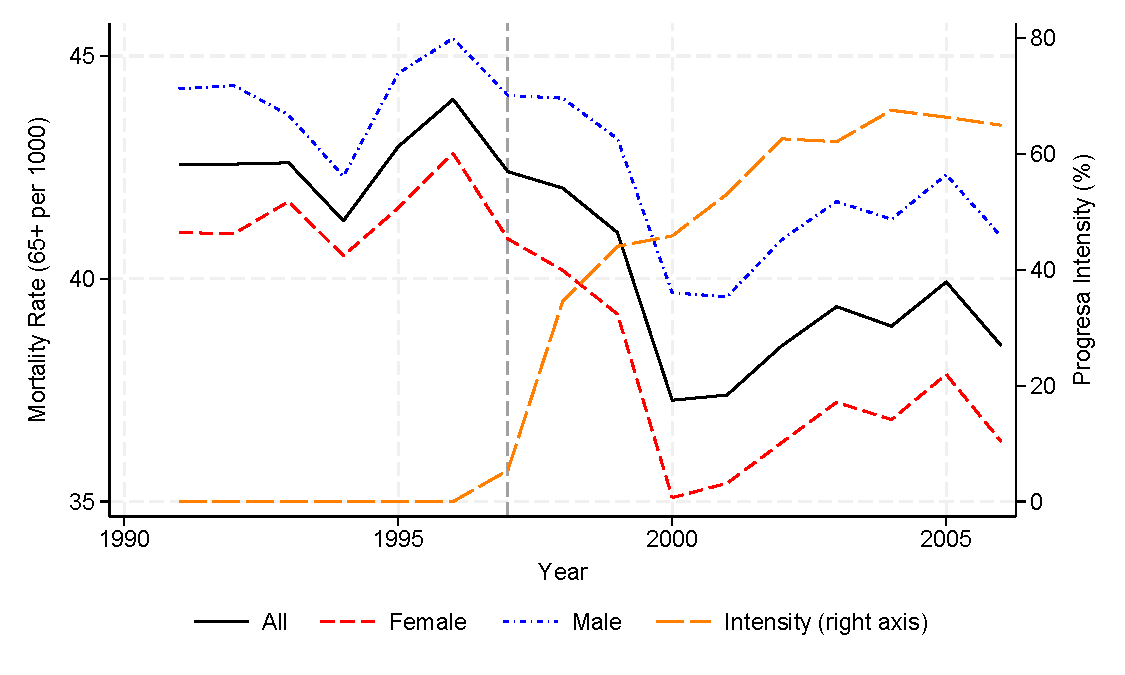
\includegraphics[width=0.89\textwidth, keepaspectratio]{Figure_1a_marg.pdf}
\end{figure}
\end{frame}

\note{This figure shows the key trends. The mortality rate for adults 65 and older in highly marginalized municipalities is on the left axis, and Progresa penetration is on the right. The vertical line marks 1997 when the program started. We can see that mortality was declining before the program, and enrollment grew rapidly after 1997. The identification challenge is separating the program's effect from the pre-existing trend.}

\begin{frame}{Geographic Distribution of Progresa Intensity}\label{maps}
\vspace{-2mm}
\begin{columns}
  \begin{column}{0.5\textwidth}
    \centering
    {(a) Intensity in 1999 (early phase)}\\
    \vspace{2pt}
    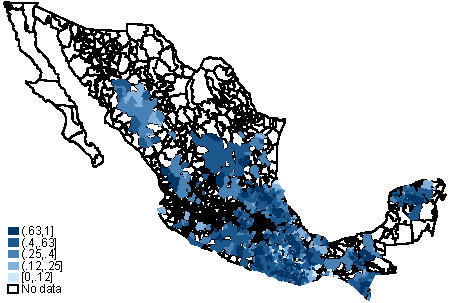
\includegraphics[width=\textwidth, keepaspectratio]{Figure_1b_inten1999.pdf}
  \end{column}
  \begin{column}{0.5\textwidth}
    \centering
    {(b) Intensity in 2005 (later phase)}\\
    \vspace{2pt}
    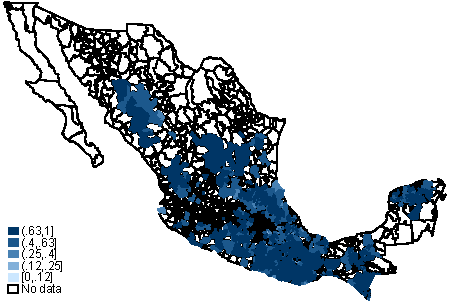
\includegraphics[width=\textwidth, keepaspectratio]{Figure_1c_inten2005.pdf}
  \end{column}
\end{columns}
% \vspace{2mm}
% {\footnotesize Municipality-level Progresa intensity (share of beneficiary households) among highly marginalized municipalities. Darker shading = higher intensity. Substantial variation across municipalities in both phases motivates the two-phase DiD design.}
\end{frame}

\note{These maps show the geographic distribution of Progresa intensity in 1999 and 2005. There is substantial variation across municipalities in both phases, and the geographic pattern shifts between early and late enrollment. This variation is what we exploit in the analysis.}

%%%%%%%%%%%%%%%%%%%%%%%%%%%%%%%%%%%%%%%%
%%% EMPIRICAL STRATEGY %%%
%%%%%%%%%%%%%%%%%%%%%%%%%%%%%%%%%%%%%%%%
\section{Empirical Strategy}

\begin{frame}{Empirical Strategy: Difference-in-Differences}\label{empirics}
\small



\begin{itemize}
  \item \textbf{Early phase} (1997--1999): $\textit{Intensity}_{m,1999}$ --- share of households enrolled by 1999
  \item \textbf{Late phase} (2000--2005): $\textit{Intensity}_{m,2005}$ --- share enrolled by 2005
  \item After 2005, expansion shifted toward urban areas $\to$ two phases are largely non-overlapping
\end{itemize}

\vspace{6pt}

\textbf{Baseline specification}

\vspace{-2pt}

\begin{equation*}
\text{MR}_{m,t}
= \beta_{0}\,\textit{Post}_{t} \times \textit{Intensity}_{m,1999}
+ \beta_{1}\,\textit{Post}_{t} \times \textit{Intensity}_{m,2005}
+ \delta_{m} + \gamma_{t} + \chi_{m,t} + \varepsilon_{m,t}
\end{equation*}

\vspace{4pt}

\begin{itemize}
  \item $\text{MR}_{m,t}$: deaths per 1,000 inhabitants aged $65+$, municipality $m$, year $t$
  \item $\textit{Post}_{t}$: $= 1$ for years $1997$--$2006$; $\delta_m$, $\gamma_t$: municipality and year fixed effects
  \item $\chi_{m,t}$: Seguro Popular enrollment intensity (controls for confounding health insurance rollout)
  \item \textbf{Coefficient of interest}: $\beta_0$ --- effect of early-phase enrollment intensity on elderly mortality
  \item SE clustered at the municipality level; weighted by elderly population
\end{itemize}

\end{frame}

\note{Our identification strategy compares municipalities that enrolled more households in the early phase of Progresa (1997-1999) with those that enrolled more in the late phase (2000-2005). The post indicator turns on in 1997. We control for Seguro Popular, Mexico's public health insurance that rolled out after 2002, and weight by the elderly population to avoid giving outsized influence to tiny, volatile municipalities.}

\begin{frame}{Event Study Specification}\label{eventstudy_spec}
\small

\vspace{2pt}
\begin{equation*}
\text{MR}_{m,t}
= \sum_{k \neq 1996} \beta_{k}\,\mathbf{1}[t=k] \times \textit{Intensity}_{m,1999}
+ \sum_{k \neq 1996} \theta_{k}\,\mathbf{1}[t=k] \times \textit{Intensity}_{m,2005}
+ \delta_{m} + \gamma_{t} + \chi_{m,t} + \varepsilon_{m,t}
\end{equation*}

\vspace{4pt}

\begin{itemize}
  \item Reference year: 1996 (last pre-program year)
  \item $\beta_k$ traces the effect of early-phase enrollment intensity on mortality in each year
  \item \textbf{Pre-trends test}: $\beta_k = 0$ for $k < 1997$ supports parallel trends assumption
  \vspace{4pt}
  \item \textbf{Identification assumption:} conditional on municipality and year FEs, municipalities with higher $\textit{Intensity}_{1999}$ would have followed parallel mortality trends in the absence of the program
    \begin{itemize}
      \item Restriction to highly marginalized municipalities makes this more credible: all are targeted; they differ only in speed and intensity of enrollment
    \end{itemize}
\end{itemize}

\end{frame}

\note{The event study lets us look year by year and test whether pre-trends were parallel. The reference year is 1996. If municipalities that ended up with more Progresa enrollment already had different mortality trends before the program started, the parallel trends assumption would be violated, and our DiD estimates would be unreliable.}

%%%%%%%%%%%%%%%%%%%%%%%%%%%%%%%%%%%%%%%%
%%% RESULTS %%%
%%%%%%%%%%%%%%%%%%%%%%%%%%%%%%%%%%%%%%%%
\section{Results}

\begin{frame}{Event Study: Effect on Elderly Mortality by Sex}\label{es_main}
\vspace{-3mm}
\begin{figure}
  \centering
  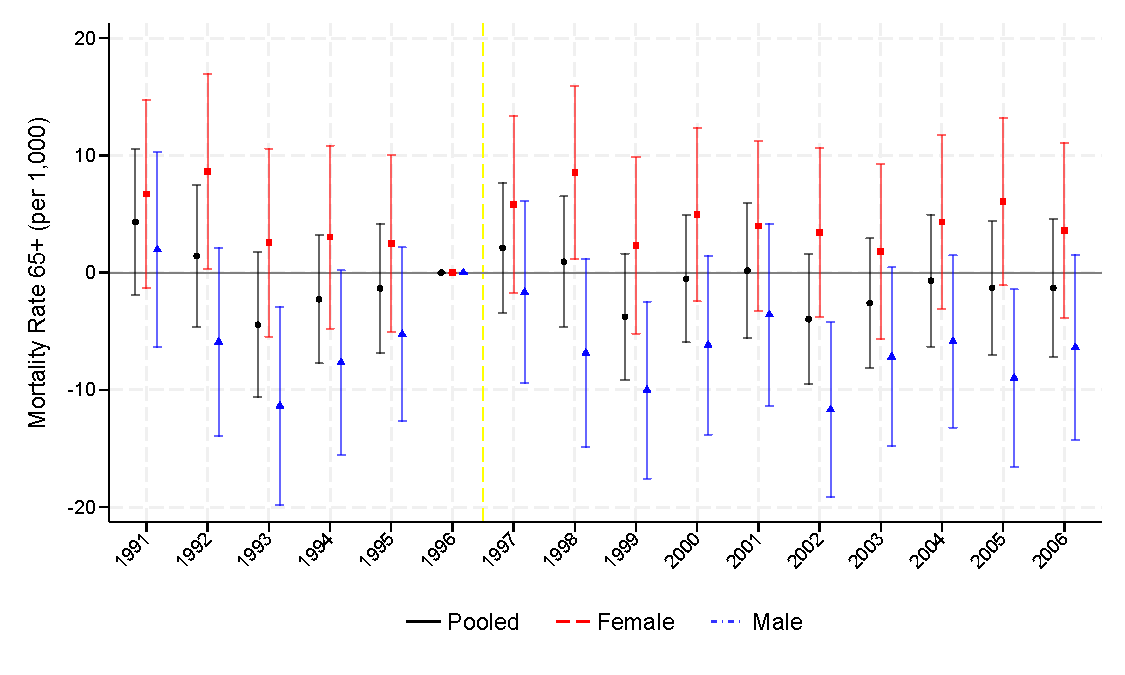
\includegraphics[width=0.85\textwidth, keepaspectratio]{Figure_2_w.pdf}
\end{figure}
% \vspace{-3mm}
% {\footnotesize Event study for early-phase Progresa intensity. Weighted by elderly population; includes Seguro Popular controls. Reference year: 1996. Sample: highly marginalized municipalities. 95\% CI shown.}
\end{frame}

\note{The event study shows the year-by-year coefficients. For females, the pre-period is relatively flat and the post-period coefficients hover around zero. For males, we see some individually significant negative coefficients in the post-period, but they are not consistent with a clean break at 1997, and they are not persistent. The average DiD estimate in the table is null for both sexes.}

\begin{frame}{Main Results: Effect on Elderly Mortality Rate}\label{main_results}
\vspace{0.4cm}
\begin{center}
\small
\begin{tabular}{lccc}
\toprule\toprule
 & Pooled & Females & Males \\
 & (1) & (2) & (3) \\
\midrule
\textit{Intensity 1999 $\times$ post} & $-0.719$ & $0.620$ & $-2.206$ \\
 & $(1.464)$ & $(1.824)$ & $(1.735)$ \\[4pt]
\textit{Intensity 2005 $\times$ post} & $-2.796$ & $-5.641^{**}$ & $0.201$ \\
 & $(1.803)$ & $(2.205)$ & $(1.994)$ \\[4pt]
Mean dep.\ var.\ (1991--1996) & $46.47$ & $46.11$ & $47.26$ \\
Observations & $17{,}904$ & $17{,}904$ & $17{,}904$ \\
No.\ Municipalities & $1{,}119$ & $1{,}119$ & $1{,}119$ \\
\midrule
Seguro Popular & Y & Y & Y \\
Weights & Y & Y & Y \\
Mean Intensity 1999 (\%) & $44.4$ & $44.4$ & $44.4$ \\
\bottomrule\bottomrule
\end{tabular}
\end{center}
\end{frame}

\note{Across all four columns, the effect of early-phase Progresa intensity on elderly mortality is small and statistically insignificant. This holds for the pooled sample, for females, and for males. Adding Seguro Popular controls doesn't change the result. Weighting doesn't change the result. The null finding is consistent across specifications.}



\begin{frame}{Cause-of-Death Analysis}\label{cod}
\small
\begin{itemize}
  \item[$\circ$] Prior work suggests mortality reductions through \textit{specific} causes (diabetes, CVD, Infect.)
  \vspace{4pt}
  \item[$\circ$] We decompose into 9 causes: cancer, cardiovascular, respiratory, infectious disease, diabetes, nutritional, ill-defined, accidents, other
  \vspace{4pt}
  \item[$\circ$] Individually significant point estimates (before multiple-testing correction):
    \begin{itemize}
      \item \textcolor{blue1}{Cancer}: $-0.887$ ($p<0.01$)
      \item \textcolor{blue1}{Ill-defined causes}: $-0.574$ ($p<0.01$)
      \item \textcolor{blue1}{Diabetes}: $-0.508$ ($p<0.05$)
      \item \textcolor{redUT}{Cardiovascular}: $+1.530$ ($p<0.10$)
    \end{itemize}
  \vspace{4pt}
  \item[$\circ$] \textbf{After Romano-Wolf step-down correction} for 9 simultaneous hypotheses:
    \begin{itemize}
      \item All adjusted $p$-values $> 0.05$ \textbf{except cancer} $\to$ other individually significant estimates likely reflect multiple-testing variation
    \end{itemize}
  \vspace{4pt}
  \item[$\circ$] The ``ill-defined causes'' result warrants additional caution: likely reflects \textit{changes in cause-of-death coding}, not true mortality reductions
  \vspace{4pt}
  \item[$\circ$] Event study plots show broad pre/post overlap for most causes: \textbf{no visual break at 1997}
\end{itemize}
\end{frame}

\note{We also looked at cause-specific mortality. Before correcting for multiple testing, we find some significant estimates — cancer, ill-defined causes, and diabetes go down; cardiovascular goes up. But once we apply the Romano-Wolf correction for testing nine hypotheses jointly, almost none survive. The ill-defined cause result is especially suspicious because it may just reflect better death certificate coding over time. The cause-specific event studies show no consistent break at the program rollout date.}

%%%%%%%%%%%%%%%%%%%%%%%%%%%%%%%%%%%%%%%%
%%% ROBUSTNESS %%%
%%%%%%%%%%%%%%%%%%%%%%%%%%%%%%%%%%%%%%%%
\section{Robustness}

\begin{frame}{Robustness: Functional Form}\label{robustness_ff}
\small
\begin{itemize}
  \item[$\circ$] Main result (levels) is robust across alternative functional forms:
    \vspace{4pt}
    \begin{enumerate}
      \item \textbf{Log mortality rate} --- similar coefficients, avoids large-municipality dominance
      \vspace{4pt}
      \item \textbf{Poisson with raw death counts} --- handles zero-mortality municipality-year cells; addresses \smallcite{ChenRoth2024QJE} concerns about log with zeros
      \vspace{4pt}
      \item \textbf{Age-Adjusted Mortality Rate (AAMR)} --- directly standardizes for municipal age structure
    \end{enumerate}
  \vspace{8pt}
  \item[$\circ$] All specifications: estimates remain \textbf{small and statistically insignificant}
  \vspace{8pt}
  \item[$\circ$] Event study patterns qualitatively similar across functional forms
  \vspace{8pt}
  \item[$\circ$] We report levels in the main analysis for interpretability (deaths per 1,000) and comparability with prior literature
\end{itemize}
\end{frame}

\note{We checked whether our null finding depends on how we define the outcome. Whether we use log mortality rates, Poisson regression with raw death counts, or age-adjusted mortality rates, the result is the same: small, insignificant effects. The event study patterns look qualitatively similar across all specifications.}

\begin{frame}{Replicating Barham \& Rowberry (2013)}\label{br_replication}
\small

\textbf{Original BR design:} mortality regressed on a time-varying two-year lagged enrollment intensity
\begin{equation*}
\text{MR}_{m,t} = \alpha_0 + \alpha_1\,\textit{Intensity}_{m,t-2} + \delta_m + \gamma_t + \chi_{m,t} + \varepsilon_{m,t}
\end{equation*}

\vspace{8pt}

\begin{columns}[T]
  \begin{column}{0.52\textwidth}
    \textbf{Sensitivity of BR's estimate:}
    \vspace{4pt}
    \begin{itemize}
      \item[\textbf{(A)}] BR original: $-6.37$ deaths/1,000 ($p<0.01$)
      \item[\textbf{(B)}] Our close replication: $-7.06$ deaths/1,000 ($p<0.01$)
      \vspace{4pt}
      \item[\textbf{(C)}] Add \textit{population weights}: attenuates $\approx$\textbf{47\%} to $-3.74$ deaths/1,000 ($p<0.01$)
      \vspace{4pt}
      \item[\textbf{(D)}] 1-year lag $+$ weights: $-3.46$ deaths/1,000 ($p<0.01$)
      \vspace{4pt}
      \item[\textbf{(E)}] 3-year lag $+$ weights: $-2.07$ deaths/1,000 ($p<0.01$)
    \end{itemize}
  \end{column}
  \begin{column}{0.46\textwidth}
    \textbf{Why does weighting matter?}
    \vspace{4pt}
    \begin{itemize}
      \item[$\circ$] Progresa targeted most isolated, smallest, poorest communities first
      \item[$\circ$] These have highest intensity \textit{and} most volatile mortality rates (small populations)
      \item[$\circ$] Unweighted: excess influence to smallest municipalities
      \item[$\circ$] Weighting by elderly population: each municipality weighted proportional to its contribution to total deaths
    \end{itemize}
  \end{column}
\end{columns}

\vspace{6pt}
% \textit{Key takeaway: the short-run result is sensitive to choices that are not driven by the data.}

\end{frame}

\note{BR's original estimate is -6.37 deaths per 1,000, and we replicate it closely at -7.06. When we add population weights, the estimate drops by nearly half to -3.74 — still statistically significant but substantially smaller. Switching to a three-year lag (also with weights) brings it down further to -2.07, still significant at p<0.01. These are all equally defensible choices. The key lesson is that the short-run result is sensitive to specification, and the magnitude shrinks substantially.}

\begin{frame}{Adapting the BR Design to Our Framework}\label{br_adapt}
\small

\textbf{Our adapted design:} replaces time-varying lagged intensity with fixed early-phase intensity $\times$ post indicator
\begin{equation*}
\text{MR}_{m,t} = \beta_0\,\textit{Post}_t \times \textit{Intensity}_{m,1999} + \delta_m + \gamma_t + \varepsilon_{m,t}
\end{equation*}

\vspace{6pt}

\begin{itemize}
  \item[$\circ$] \textbf{Advantage:} enables pre-trends test (BR's design did not allow this)
  \item[$\circ$] \textbf{BR sample, unweighted:} estimate $\approx -4.0$ deaths/1,000 ($p<0.01$)
  \item[$\circ$] \textbf{BR sample, with population weights:} $-1.66$ deaths/1,000 ($p<0.05$) $\to$ attenuates $\approx$58\% relative to unweighted
  \item[$\circ$] \textbf{Full highly marginalized sample:} not statistically significant in any specification
  \vspace{6pt}
  \item[$\circ$] \textbf{Event study reveals additional concern for BR sample}
    % \begin{itemize}
    %   \item Males in BR sample: \textcolor{redUT}{clear pre-trend violations} before 1997
    %   \item Females in BR sample: post-program coefficients do not show consistent break from pre-period
    % \end{itemize}
  \vspace{6pt}
  \item[$\circ$] \textbf{Conclusion:} short-run effect sensitive to sample and design; full HM sample shows no significant effect
\end{itemize}

\end{frame}

\note{When we apply our pre/post framework to the BR sample, we can now run the event study they couldn't. For males in their sample, there are clear pre-trends — the identification assumption is likely violated. For females, the post-period doesn't show a consistent break. The weighted estimate is -1.66, significant at 5\% but 58\% smaller than the unweighted counterpart. In the full highly marginalized sample there is no significant effect at all.}

\begin{frame}{Event Study by Sex and Sample, 1992--2002}\label{fig_a6}
\vskip 2mm
\begin{figure}
  \centering
  \begin{columns}
    \begin{column}{0.5\textwidth}
      \centering {\small (a) BR Sample --- Females}\\
      \vspace{2pt}
      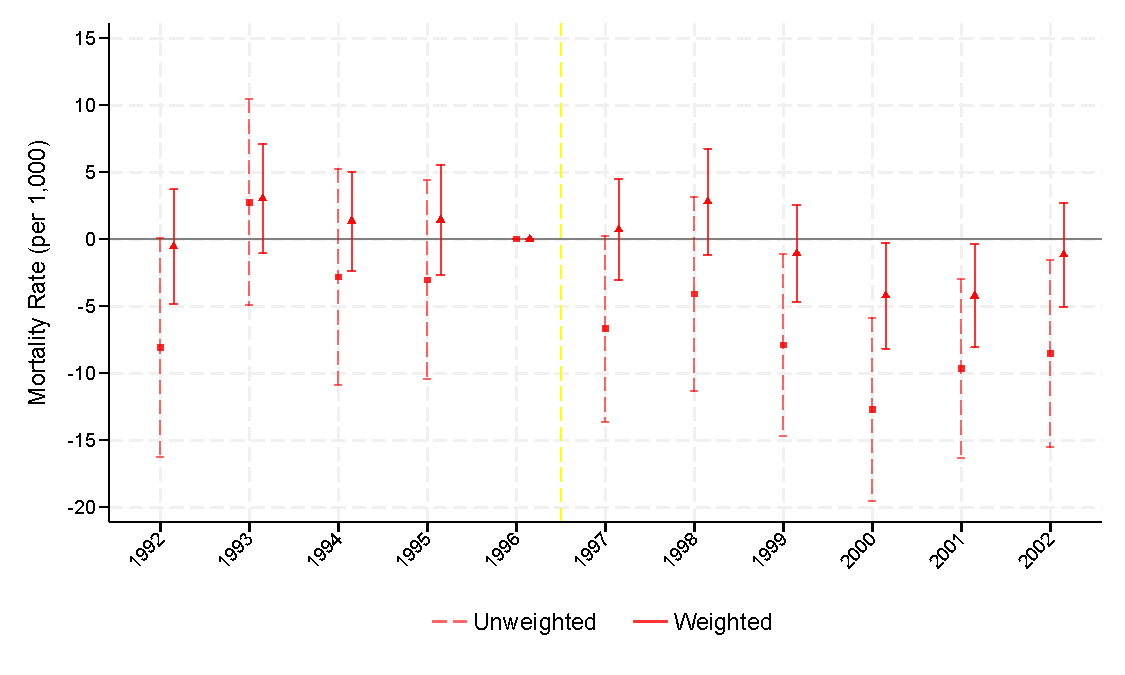
\includegraphics[width=\textwidth, height=0.38\textheight, keepaspectratio]{appendix/AF9a_F6_emr65f_BR.pdf}
    \end{column}
    \begin{column}{0.5\textwidth}
      \centering {\small (b) High Marginalization --- Females}\\
      \vspace{2pt}
      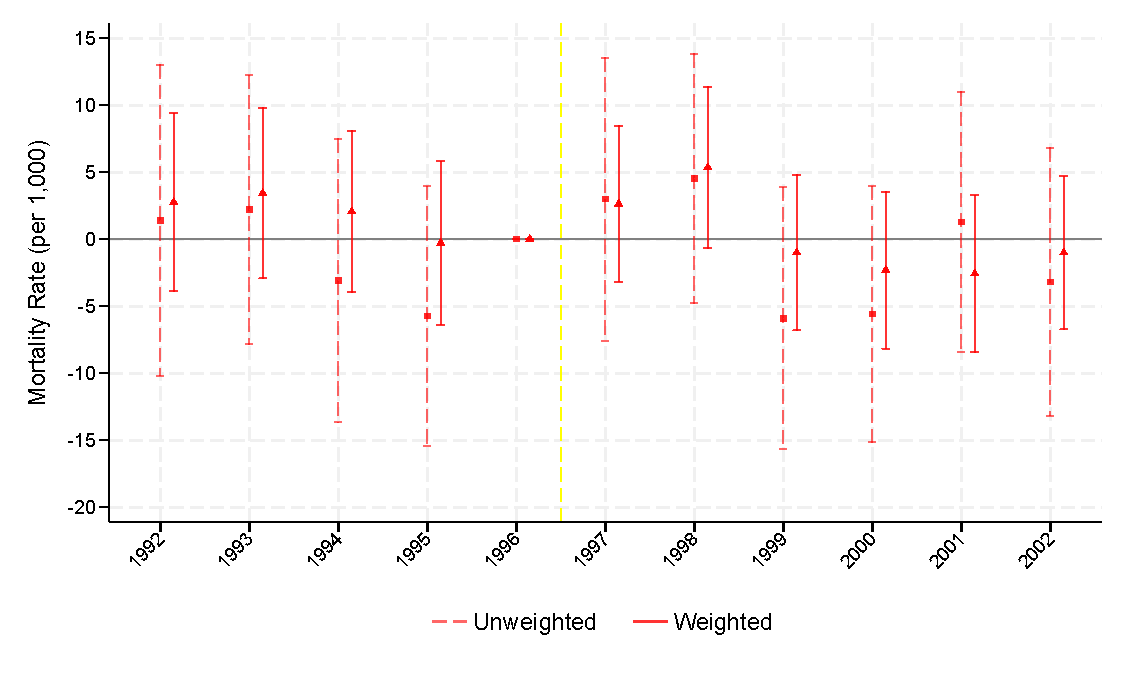
\includegraphics[width=\textwidth, height=0.38\textheight, keepaspectratio]{appendix/AF9b_F6_emr65f_HighMarg.pdf}
    \end{column}
  \end{columns}
  \begin{columns}
    \begin{column}{0.5\textwidth}
      \centering {\small (c) BR Sample --- Males}\\
      \vspace{2pt}
      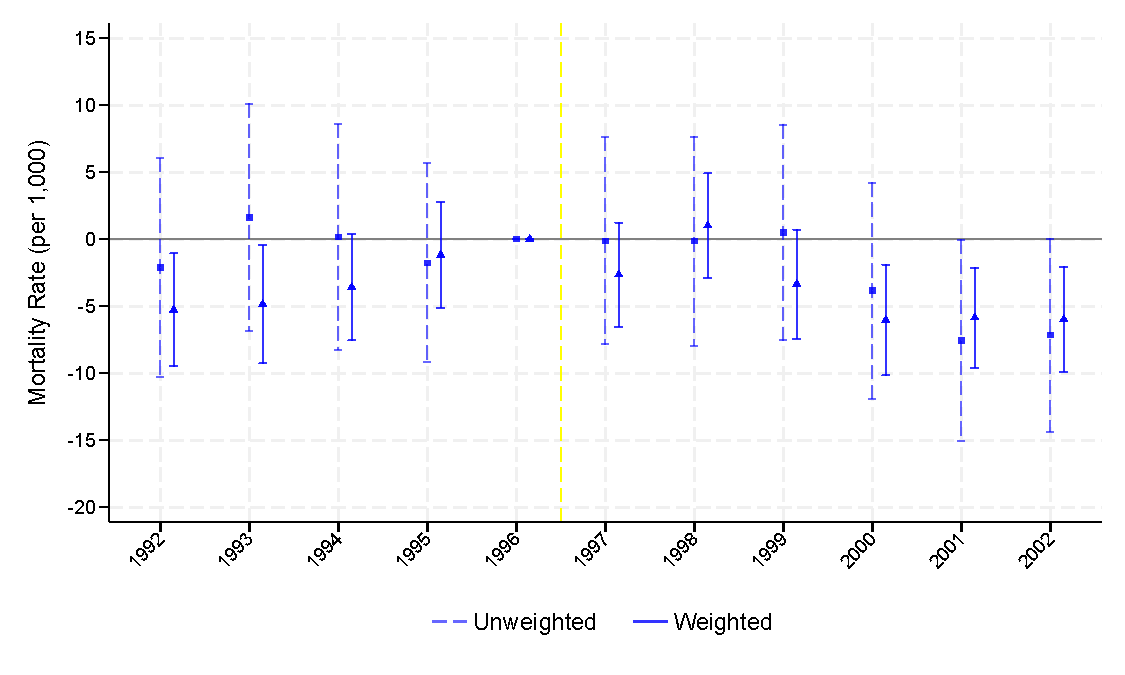
\includegraphics[width=\textwidth, height=0.38\textheight, keepaspectratio]{appendix/AF9c_F6_emr65m_BR.pdf}
    \end{column}
    \begin{column}{0.5\textwidth}
      \centering {\small (d) High Marginalization --- Males}\\
      \vspace{2pt}
      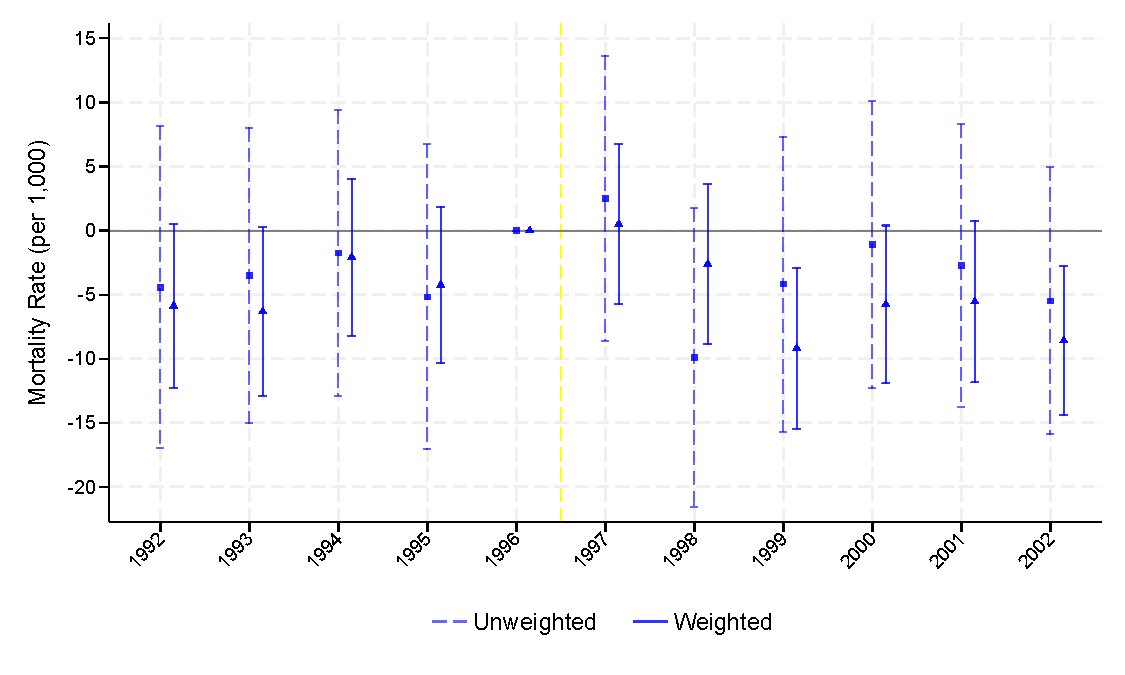
\includegraphics[width=\textwidth, height=0.38\textheight, keepaspectratio]{appendix/AF9d_F6_emr65m_HighMarg.pdf}
    \end{column}
  \end{columns}
\end{figure}
\end{frame}

%%%%%%%%%%%%%%%%%%%%%%%%%%%%%%%%%%%%%%%%
%%% MECHANISMS %%%
%%%%%%%%%%%%%%%%%%%%%%%%%%%%%%%%%%%%%%%%
\section{Mechanisms}

\begin{frame}[shrink=15]{Mechanisms: Labor Supply and Living Arrangements}\label{mechanisms_lab}
\vspace{0.2cm}
\small
\textbf{Data:} Progresa experimental evaluation (ENCASEH 1997; ENCEL 1998--2000). Sample: elderly $65+$ in eligible households in 506 treatment and 320 control localities.

\vspace{4pt}

\textbf{Specification:}
\vspace{-4pt}
\begin{equation*}
Y_{ij,t} = \alpha + \beta_t + \gamma\,\mathbbm{1}[\text{Treatment}]_i + \delta_t\,\mathbbm{1}[\text{Treatment}]_i + \mu_m + \varepsilon_{ij,t}
\end{equation*}
\begin{center}
\begin{table}
  \centering
  \scriptsize
  \begin{threeparttable}
    
\begin{tabular}{lcccc}
\toprule
 & (1) & (2) & (3) & (4) \\
 & Weekly Hours & Live Alone & With Children & Only Elderly \\
\midrule
\multicolumn{5}{l}{\textbf{Panel A: Females}} \\
\midrule
Treat $\times$ 1998 & 0.124 & 0.000 & 0.001 & $-$0.008 \\
                    & (1.136) & (0.008) & (0.011) & (0.008) \\[4pt]
Treat $\times$ 1999 & 0.292 & 0.007 & 0.015 & 0.012 \\
                    & (1.070) & (0.010) & (0.018) & (0.014) \\[4pt]
Observations        & 3,338 & 3,597 & 3,597 & 3,597 \\
Control Mean (1997) & 3.923 & 0.044 & 0.708 & 0.145 \\
\midrule
\multicolumn{5}{l}{\textbf{Panel B: Males}} \\
\midrule
Treat $\times$ 1998 & $-$1.210 & 0.012 & $-$0.008 & $-$0.007 \\
                    & (1.895) & (0.008) & (0.011) & (0.010) \\[4pt]
Treat $\times$ 1999 & 0.378 & 0.008 & 0.040$^{**}$ & $-$0.001 \\
                    & (1.872) & (0.012) & (0.020) & (0.017) \\[4pt]
Observations        & 3,170 & 3,419 & 3,419 & 3,419 \\
Control Mean (1997) & 25.288 & 0.049 & 0.676 & 0.159 \\
\bottomrule
\end{tabular}

  \end{threeparttable}
\end{table}
\end{center}

\end{frame}

\note{Using the experimental data, we test directly whether Progresa changed elderly labor supply or living arrangements. The answer is no on both counts. Elderly people didn't work fewer hours, and they didn't become more or less likely to live with children or alone.}

\begin{frame}{Mechanisms: Conclusions}\label{mechanisms_enigh}
\small

\textbf{Experimental evidence (labor supply \& living arrangements):}
\begin{itemize}
  \item[$\circ$] \textbf{Labor supply:} no significant change in elderly weekly hours worked
  \item[$\circ$] \textbf{Living arrangements:} no change in probability of living alone, with children, or with elderly only
  \item[$\circ$] Null on living arrangements \textbf{rules out the informal-caregiving pathway}
\end{itemize}

\vspace{6pt}

\textbf{Income \& nutrition (ENIGH, 1992--2006):}
\begin{itemize}
  \item[$\circ$] Outcomes: labor income; food spending (cereals, meat/dairy, vegetables, fats/sugar); health spending
  \item[$\circ$] All coefficients imprecise $\to$ no significant behavioral responses detected
  \item[$\circ$] Consistent with experimental null; limited power given survey design, but direction reinforces it
\end{itemize}

\vspace{6pt}

\textbf{Overall:} two independent data sources converge --- none of the channels through which \textit{Progresa} could reach the elderly were activated at detectable levels. The null mortality result is \textbf{interpretable}, not just a power issue.

\end{frame}

\note{Slide 17 showed the experimental results — no changes in labor supply or living arrangements. Here we add the ENIGH findings: no significant effects on income, food consumption, or health spending either. The two data sources tell the same story. The null mortality result is not surprising given that none of the mechanisms were activated.}

% \begin{frame}{Mechanisms: Summary}\label{mechanisms_summary}
% \small
% \begin{columns}[T]
%   \begin{column}{0.48\textwidth}
%     \textbf{Three channels tested}
%     \vspace{6pt}
%     \begin{enumerate}
%       \item \textbf{Health conditionality} \\
%         One annual clinic visit \\[4pt]
%         {\footnotesize $\to$ \smallcite{BehrmanParker2013Demography}: increased utilization \\
%         $\to$ \smallcite{aguila2024conditional}: \textcolor{redUT}{no improvement in biomarkers} \\
%         $\to$ Cause-of-death analysis: no significant reduction in cardiovascular or infectious disease \\
%         \textbf{Conclusion: partially activated, clinically ineffective}}
%       \vspace{8pt}
%       \item \textbf{Income and nutrition} \\
%         {\footnotesize ENIGH analysis: \textcolor{redUT}{no detectable response} \\
%         \textbf{Conclusion: not activated}}
%       \vspace{8pt}
%       \item \textbf{Living arrangements} \\
%         {\footnotesize Experimental data: \textcolor{redUT}{no change in co-residence} \\
%         \textbf{Conclusion: not activated}}
%     \end{enumerate}
%   \end{column}
%   \begin{column}{0.48\textwidth}
%     \textbf{The bigger picture}
%     \vspace{6pt}
%     \begin{itemize}
%       \item[$\circ$] The null is \textbf{interpretable}, not just a power issue
%       \vspace{4pt}
%       \item[$\circ$] Contrast with \textbf{direct pension programs}:
%         \begin{itemize}
%           \item \textit{70 y Más} (direct, unconditional pension to $70+$): $-5.5\%$ elderly women mortality \smallcite{jeon2025short}
%           \item Chile's basic solidarity pension: $-2.7$ pp four-year mortality \smallcite{MiglinoNavarrete2023AEJP}
%         \end{itemize}
%       \vspace{4pt}
%       \item[$\circ$] Key difference: when income goes \textbf{directly to the elderly}, no need for intergenerational redistribution within the household
%       \vspace{4pt}
%       \item[$\circ$] When income goes to mothers via a child-focused CCT, elderly members depend on household redistribution that may not occur
%     \end{itemize}
%   \end{column}
% \end{columns}
% \end{frame}

\note{Here's the bottom line on mechanisms. The health conditionality reached elderly people in terms of clinic visits, but didn't improve biomarkers or cause-specific mortality. Income and living arrangements were not changed. The null is coherent and interpretable. And it stands in stark contrast to direct pension programs, where income goes straight to the elderly and mortality effects are found. The intermediation through the household is what makes the CCT different.}

%%%%%%%%%%%%%%%%%%%%%%%%%%%%%%%%%%%%%%%%
%%% CONCLUSION %%%
%%%%%%%%%%%%%%%%%%%%%%%%%%%%%%%%%%%%%%%%
\section{Conclusion}

\begin{frame}{Concluding Remarks}\label{conclusion}
\small
\begin{itemize}
  \item[$\circ$] \textbf{Main finding:} \textit{Progresa} had \textbf{no significant effect} on elderly mortality ($65+$) over its first ten years of operation
    \begin{itemize}
      \item Robust to weighting, functional form, and Seguro Popular controls
      \item Result holds for pooled sample, females, and males separately
    \end{itemize}
  \vspace{4pt}
  \item[$\circ$] \textbf{Short-run evidence revisited:} the \smallcite{BarhamRowberry2013JDE} estimate is sensitive to specification
    \begin{itemize}
      \item Population weighting attenuates the effect by $\approx 50\%$
      \item Alternative lag structures further reduce it
      \item Event study reveals pre-trend violations in the BR sample for males
    \end{itemize}
  \vspace{4pt}
  \item[$\circ$] \textbf{Mechanisms:} income, nutrition, and caregiving channels not detectably activated
    \begin{itemize}
      \item Clinic utilization increased but no biomarker improvement \smallcite{aguila2024conditional}
    \end{itemize}
  \vspace{4pt}
  \item[$\circ$] \textbf{Policy implication:} CCTs structured around children's education do not reliably deliver mortality benefits to elderly household members
    \begin{itemize}
      \item Programs transferring resources \textit{directly} to the elderly are more effective for reducing elderly mortality \smallcite{Menares2026JHR, MiglinoNavarrete2023AEJP}
    \end{itemize}
\end{itemize}
\end{frame}

\note{To summarize: we find no evidence that Progresa reduced elderly mortality over ten years. The earlier short-run positive finding is sensitive to specification choices that are equally defensible. The behavioral channels that would produce a mortality effect were not activated. The policy lesson is that if you want to reduce elderly mortality, you need programs that put money directly in the hands of older adults — not child-focused CCTs that rely on intergenerational redistribution.}



\begin{frame}[noframenumbering, plain]
\begin{center}
\Huge{\color{Blue}Thank you!} \\[12pt]
\small{
  Felipe Menares \\
  \texttt{felipeme@iadb.org} \\[8pt]
  \textcolor{gray}{All data publicly available from INEGI}
}
\end{center}
\end{frame}

{\tiny\bibliography{bibliography}}

\includepdf[pages={2},noautoscale=false,fitpaper=false]{ppt_iadb/Half-baked_Lunch_Backdrop.pdf}
\end{document}
